%%%%%%%%%%%%%%%%%%%%%%%%%%%%%%%%%%%%%%%%%%%%%%%%
\section{Statistical Shape Model}
\label{sec:5_SSM}

In a first step, we propose to use the correspondence relation between the database meshes to construct statistical shape models. These latter are a common application for meshes in correspondence. They enable the analysis of shapes distribution by describing the main variations among a class. They can be used for various operations: for example the characterization of the main shape variations among a population allows a better understanding of the shapes studied. The statistical models are also often used as prior knowledge for image segmentation, which allows more stable and precise results. They can also be used to retrieve 3D information from 2D images using the additional knowledge of the model. 

In all of these applications, the accuracy of the model is critical. We endeavor to create statistical models that should be convenient and reliable and measure their limits. They can afterwards be used for any aforementioned application, once their expected accuracy is established. 
We especially propose to work with Gaussian Process Morphable Models (GPMMs), an extension of PCA-based SSMs, that have been little used by now. In particular, to the best of our knowledge, they have never been used for wrist bones encoding. The additional computation of PCA-based SSMs have two purposes: it enables comparison with GPMMs and it is required for the computation of correspondence quality criteria. 

The section starts with a brief state-of-the-art of existing statistical shape models. Then PCA-based SSMs are computed and analyzed, both models describing individual bones and a model characterizing the whole wrist at once. Then a more complex statistical model is used, based on Gaussian Processes, and the practicality of such a model for our data is discussed. 

%======================================
\subsection{State of the art}
\label{subsec:4_SSM_SoA}


%With computers come the will and need to automate as many tasks as possible, with the most accurate outcomes achievable. One of the great goals of computer scientists has been since quite early the automation of image interpretation. One key step to achieve it is the ability to recognize and delineate objects in pictures. Yet in a same class of objects, shapes change over instances, and sometimes instances themselves transform over time. 
One challenge in computer science is to make the machines able to recognize and delineate objects in pictures. Yet, objects can be appear very different depending on the camera angle, or due to differences of shapes between instances. It is especially the case in medical imaging, every subject's organs are uniquely shaped, and they evolve over time, whether fast, such as beating hearts or more slowly. The need to adapt an initial object to the shape of the considered instance has risen. 


Different solutions were proposed over time to segment variously shaped instances of the same class of objects. Model-based segmentation is a top-down approach consisting in matching a model containing information about the class expected shape with new images. It is one of the most successful existing methods, the prior information brought by the model provides stability against image artifacts and perturbations \cite{heimann_2009_statistical}. The flexibility of the model enables adaptation to the various instances of the class. We focus on this segmentation approach. 

One of the first flexible model was introduced by Kass et al. \cite{kass_1988_snakes} and is called Active Contour Models or Snakes. It consists in describing the contour of an object as a continuous spline subjected to forces controlling compliance to image features and fulfillment of structural constraints such as smoothness. However, snakes lack specificity as they don't incorporate knowledge about shape variations in the class and are not restrained in their distortions as long as the energies are minimized \cite{davies_2008_statistical}. 

Information about common variations need to be added in the model. One straight-forward approach consists in considering multiple instances of the object class as training shapes and learning from the set statistical properties of the class \cite{heimann_2009_statistical}. It leads to Statistical Shape Models (SSMs), most of them being based on a Principal Component Analysis (PCA), which is further detailed in \secref{subsec:4_PCA}. The first SSM was introduced by Cootes et al. in \cite{cootes_1994_use} and was more detailed later in \cite{cootes_1995_active}. The statistical analysis of the training set is computed using PCA: they work with shapes described by landmarks, and analyze the points positions distribution over instances. This distribution is called Point Distribution Model (PDM). The model based on the PDM used for image segmentation is named Active Shape Model. Another popular SSM was introduced by Blanz and Vetter, called the Morphable Model. It is used for generation of new human faces and extraction of a 3D mask from a 2D picture, also based on PCA \cite{blanz_1999_morphable}.

PCA-based models are linear, which makes them mathematically easy and fast to compute. They can only represent linear combinations of the training shapes, which makes them robust towards artifacts and noise \cite{luthi_2017_gaussian}. However this limitation to the linear span defined by the training set is both an advantage and a downside of the method. It prevents the apparition of impossible shapes, but it also prevents the model from generating accurate shapes too different from the training set. To overcome this problem, the training data should be as numerous and various as possible. 

For PCA-based models, the training set should ideally be very large, however this is often not possible, in particular when working with medical images. Therefore, works have been conducted to reduce the impact of limited quantity of data for the model creation. Artificial training data can be used, as in \cite{cootes_1995_combining}. Cootes et al propose to add artificial training data using finite element models (FEM). These latter give a set of linear deformations of one shape corresponding to its modes of vibration. They generate many new shapes using FEM on every instance of the training set, and use all original and generated shapes to train the SSM. However, the variations of the FEMs are arbitrary and may not be representatives of the real variations of the class of shapes. In order to extend the flexibility of the model, a spatial partition of the object can also be a solution, as proposed by Zhao et al in \cite{zhao_2005_partitioned}. They partition shapes in tiles, and apply a PCA to each tile separately, before projecting the results in one hyperspace to ensure coherence between the fragments. 
Blanz and Vetter \cite{blanz_1999_morphable} propose a similar partitioning of the total shape in sub-regions, which were morphed individually before being blended back together. Finally, another solution consists in decomposing the shapes in the frequency domain as proposed by Davatzikos et al \cite{davatzikos_2003_hierarchical}, and later improved by Nain et al. \cite{nain_2007_multiscale}. The hierarchical multi-scale formulation of SSMs is based on a wavelet transform of the points positions. 

% PGA? 

Wang and Staib chose to improve the SSM by working on the covariance matrix, rather than on the data \cite{wang_2000_boundary}. They introduce the covariance matrix based on the PDM of the training data, but they also propose a covariance matrix describing smoothness constraint between neighboring points. Finally they combine both matrices to associate the specificity brought by the model trained on the data with the variability of the smoothness constraint. 
Lüthi et al propose in a series of articles summarized in \cite{luthi_2017_gaussian} a similar idea of SSM but extended. Their model is based on Gaussian Processes and is further detailed in \secref{subsec:4_GP}. They call it Gaussian Process Morphable Model (GPMM). The GPMM can be viewed as an extension of the PCA-based SSM, in that it is more complete. Gaussian Processes were already used in the 90's for image registration, as referred in the overview by Grenander et al. \cite{grenander_1998_computational}. Lüthi et al. argue that in their version using the Nyström approximation any combination of kernels can be used, which makes the method so powerful.  

In this state of the art, we have focused on models for shapes characterized by landmarks distributed over the object, and already in dense correspondence. It is indeed the type of data we're working with (cf chapter \ref{chap:Method}). However, different shape characterizations, such as skeletons representations, surface encoding with Spherical Harmonics or Fourier surfaces lead to diverse models. 

In the following sections, two statistical models have been implemented: a PCA-based Statistical Shape Model and a model based on Gaussian Processes. The theory behind the models, as well as the results achieved are presented and discussed. 

%======================================
\subsection{Principal Component Analysis}
\label{subsec:4_PCA}

The Principal Component Analysis, also called PCA, is a statistical procedure used to extract the principal modes of variations of data. It can also be used for dimensionality reduction of data, as will be further explained. It has been widely used for image segmentation, the PCA being used as prior information about the object class shape in the form of a Statistical Shape Model. It can have other applications, such as shape analysis by examination of the main modes of variations or investigation of the impact of some factors such as gender. Finally, as previously mentioned in Chapter \ref{chap:Method}, the SSM is a mean of measuring correspondence quality. 

We chose to apply PCA on our data. It is aimed at controlling the quality of the correspondence results previously computed. It is also meant for comparison with the Gaussian Process Morphable Model later computed. First we detail the PCA procedure (further details can be found in Jolliffe's work, for instance in \cite{jolliffe_2011_principal}). Then we explain and examine our results. 

The procedure requires multiple properties of the data: the data must follow a Gaussian distribution. In the case of coordinates of landmarks, the shapes must be previously similarly aligned, oriented and scaled, to avoid noise. We make the assumption that the bone shapes indeed follow a Gaussian distribution, which is a classical hypothesis. As explained in Chapter \ref{chap:Method}, all bones were previously aligned and scaled using ICP, this condition is met. 




%it is also possible to calculate /m and km by a singular value decomposition (SVD) on the aligned landmark matrix L ¼ ððx1  xÞ    ðxs  xÞÞ. From a computational point of view, this method is to be preferred due to the higher numerical stability. [Heimann 09] (on utilise ça quand on passe par la librairie sklearn)




% La PCA défini un ensemble d'axes orthogonaux qui maximise la quantité ... [ Taylor, Twining, Davies - Statistical models of shape, (2.15)]

% Since there are nS shapes, there are at most nS −1 non-zero eigenvalues. 

% Si dimension (3) * nombre de points > nombre de shape-1, alors we performed dimensionality reduction by llocating the directions with 0 eigenvalie that are orthogonal to the subspace spanned by the data


%--------------------------------------
\subsubsection{What is Principal Component Analysis?}
\label{ssubsec:4_PCA_what}

The Principal Component Analysis is a statistical procedure that evaluates the distribution of a set of data, and transforms them to a new space of uncorrelated components, which often leads to a dimensionality reduction. 

Let us suppose we have $n$ measurements of a vector $\mathbf{x}$ of $p$ random variables. These variables are potentially correlated. PCA transforms the data to a new space of uncorrelated variables. The axes of this new space are a set of orthogonal vectors, the origin of the coordinate system is the projection of the mean shape $\bar{\mathbf{x}}$ in the new space. 
PCA determines a set of orthogonal axes, which maximizes the variance along each axes. These axes are determined in such a way that they successively have maximum variance for the data, while being uncorrelated with previously computed axes. The number of distinct non-zero vectors is $q=\min(n-1, p)$, which often leads to a reduction of dimensionality. An example of principal components can be seen in \figref{im:4_pca_illustration}.

\begin{figure}[!ht]
	\centering
	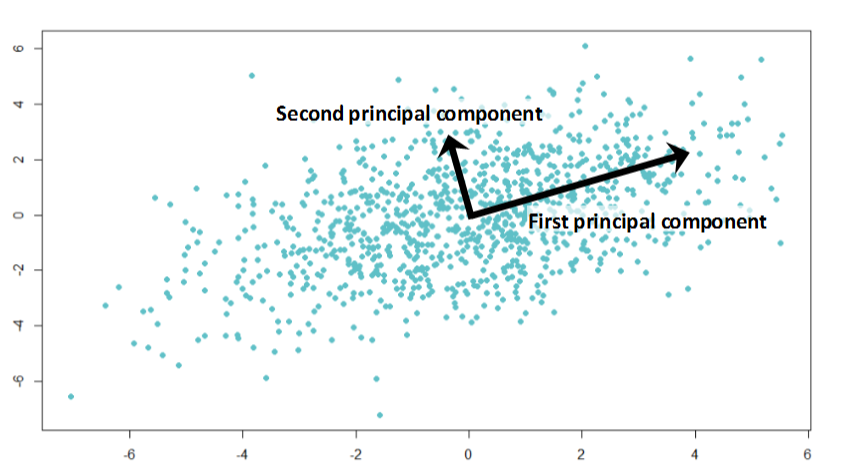
\includegraphics[width=0.8\textwidth]{\RootDir{img/pca_ex.png}}
	\caption[Example of a Principal Component Analysis]{Example of a Principal Component Analysis. The first component is the axis on which there is the most variability when the data are projected onto it. The second axis is perpendicular to the first one. The center of the new system is the center of mass of the data.}
	\label{im:4_pca_illustration}
\end{figure}

It can be proven that the orthonormal directions that maximize the variance associated to each vector are given by the eigenvectors of the data covariance matrix, corresponding to the $q$ largest eigenvalues \cite{davies_2008_statistical}. The eigenvalues give the variances associated to each eigenvector, the latter are ordered from the highest eigenvalue to the smallest one. To avoid the domination of a few high-variance variables over the others or in the case of different units, the variables are often standardized to have zero mean and unit variance \cite{jolliffe_2011_principal}. 

The PCA is computed as follows. At first the mean shape is calculated, as a simple average over the $n$ measurements.

\begin{equation}
	\label{eq:mean_vector}
	\bar{\mathbf{x}} = \frac{1}{n} \sum_{i=1}^{n} \mathbf{x_i}
\end{equation}

Let $\mathbf{X}$ be the matrix $ (n \times p)$ composed of all measurements of vector $\mathbf{x}$, and $\mathbf{X_c}$ the standardized matrix such that:

\begin{equation}
 	\mathbf{X_c}(i,j) = \frac{\mathbf{X}(i,j) - \bar{\mathbf{x}}(j)}{\sigma(\mathbf{X}(:,j))} 
 \end{equation}
 
 $\sigma(\mathbf{X}(:,j))$  is the standard deviation of the $j^{th}$ variable of all measurements of $\mathbf{x}$. 
The covariance matrix C is computed, using standardized values. 


\begin{equation}
	C = \frac{1}{n-1} \mathbf{X_c}^t \mathbf{X_c}
\end{equation}

Then, the eigenvectors matrix $V$ and their associated eigenvalues $\Lambda$ are defined such as:

\begin{equation}
	CV = \Lambda V
\end{equation}

Only the $q$ non-zero eigenvalues and their associated eigenvectors are considered. The matrix $V$ maps the data from the original space towards the new space.%, while $V^t$ allows a mapping from the new space back to the original space. 
A measurement of $\mathbf{x}$ expressed in the new base, called $x_n$, is equal to: 

\begin{equation}
	x_n = (\mathbf{x} - \bar{\mathbf{x}}) V \sqrt{\Lambda^{-1}}
\end{equation}




New measurements of $\mathbf{x}$ can be simulated by generating random vectors $w$ of size $q$, with each value $w_i \sim \mathcal{N}(0,1)$. Usually the values are forced to take their value in the interval $[-3; 3]$.
	\footnote{Let $X$ be a random variable, with a normal distribution of mean $\mu$ and standard deviation $\sigma$. Let $x$ be a value taken by $X$. Then $P(x \in [\mu -3 \sigma ; \mu +3 \sigma]) \geq 99.7\%$. Which means that almost all values that can be taken by $X$ will be in the interval $[\mu - 3\sigma ; \mu + 3\sigma]$ with a very small chance of error.
	
	We make the assumption that the distribution of $\mathbf{x}$ is a multidimensional normal distribution. The eigenvalues associated to the eigenvectors represent the variance of the modes. The square root of an eigenvalue gives the standard deviations of the mode $sd$. Then with a similar reasoning than in one dimension, with a very small error, we can define the range of all possible shapes as all those that can be described as a summation of the mean vector and the weighted eigenvectors, each weight $w_i$ being such as $w_i \in [-3; +3]$}
 The vector of size $q$ is the representation of the simulated measurement in the new space. In the original space, the simulated measurement is equal to:

\begin{equation}
	\mathbf{x_w} = \bar{\mathbf{x}} + wV^t\sqrt{\Lambda}
	\label{eq:pca_new_shape}
\end{equation}

It should be noted that the mapping are not exactly the inverse transformations of each other, even if all non-zero eigenvectors are retained, since the dimensionality of parameter space is less than the dimensionality of shape space \cite{davies_2008_statistical}. If a new observation of $\mathbf{x}$ is projected into the new space, then transformed back into the original space, it will not be strictly identical to the initial observation. Indeed the first transformation is a projection into the subspace defined by the training set, then it is transformed back through a linear interpolation of the training set measurements, using the available modes. 


Most often the last eigenvectors are associated with small variance, information added by these vectors is poor. When there are not many data, it can even be strongly linked to one of the measurement, and falsely add variance to the model, which can worsen the results. Therefore, the last eigenvectors are often ignored, and only the ones corresponding to large eigenvalues are considered. The number of eigenvectors kept can be chosen according to multiple criteria: the cumulative variance should be higher than a defined proportion of the total shape variance, for instance $95\%$ or $99\%$. Or else the number of eigenvectors kept should enable to reach a certain accuracy of data when using the model. In this case, the number $q$ of considered eigenvectors is smaller than the number of non-zeros eigenvalues. The equations are still true, $V$ and $\Lambda$ are simply replaced by their truncated versions. 


The registration of a SSM to a target shape consists in minimizing the distance between the target mesh $x_{\text{target}}$ and the deformed model $\mathbf{x_w}$. The optimization is computed over the vector $w$, which describes the weight associated to each mode. We use the mean distance $d_{\text{mean}}$ defined in \eqref{eq:mesh_dist} as the reference distance between meshes to be minimized.  


A statistical model of 3D shapes is constructed by using the position of the meshes vertices. A mesh is described by $p$ vertices in the 3D space. All coordinates are appended in a vector of size $3p$. The shapes are gathered in a matrix of size $(n \times 3p)$, with $n$ the number of available shapes. This matrix of data $\mathbf{X}$ is the one used for the PCA computation. 
The model describes the vertices location, a shape is recreated from the positions using the same edges and faces as in the training set. In the following section, such a model has been computed on our data, the results are presented. 


%--------------------------------------
\subsubsection{Application and validation}
\label{ssubsec:4_PCA_validation}

As a result of the processes applied in Chapter \ref{chap:Method}, our bones are described by 3D meshes that have been aligned, rotated and scaled in such a way that only shape differences are the cause of variations among the bones. The meshes are in dense correspondence and we make the assumption that the distribution of the bone shapes is a multidimensional normal distribution. All conditions necessary for PCA computation are met, we present a statistical model of our data.

\paragraph{Models computation}

We chose to calculate two different types of PCA: one per bone and one for the whole wrist including the 14 bones. Both models are interesting as they bring various information. A model for one bone includes less information, and can therefore be more specific and will better capture the details of the bones. Registration results will be more precise. However, if the model of the whole wrist will be less detailed, it has the benefit of considering neighboring bones altogether. The carpal bones are small and really close to each other, the shape of one necessarily influences its neighbors, the complete model takes it into account. It enables the study of how bone shapes affect each other. This hasn't been studied yet, to the best of our knowledge. 

The two main modes of variation of the whole wrist model are shown in \figref{im:4_pca_whole_wrist}. The most important variation of shape for the wrist bones is the length and thickness of the metacarpals. In the database they evolve between long and thin to shorter and thicker. It can be noted that quite logically the five of them evolve in the same way, they are all either long or short. The second most important mode of shape variation in the wrist is more subtle to observe on the illustration of \figref{im:4_pca_whole_wrist}. The radius styloid form evolves, being either further forward or backward. In the same time the extremities of the metacarpals change from being flatter and in the continuity of the bone to being more brought out. The lunate for its part present a concavity or not. The analysis of the modes of variation is interesting for a better understanding of the different types of wrists existing, and for later classification of new wrists for instance. Such analysis of the main modes of variations have been conducted for carpal bones, the bones were considered separately \cite{vandegiessen_2010_sca}.

\begin{figure}[] 
	\centering
	\begin{adjustwidth}{-.2in}{-.2in}  
		\setlength{\extrarowheight}{1em}
		\begin{tabular}{l c c }
			& \multicolumn{2}{c}{\textbf{Main Modes} } \\
			& \textbf{$\mathbf{1^{st}}$ mode (Var. $\mathbf{17\%}$)}  & \textbf{$\mathbf{2^{nd}}$ mode (Var. $\mathbf{11\%}$)}  
			\\
			
			& & \\
			
			
			\textbf{$\mathbf{-3 SD}$}
			& 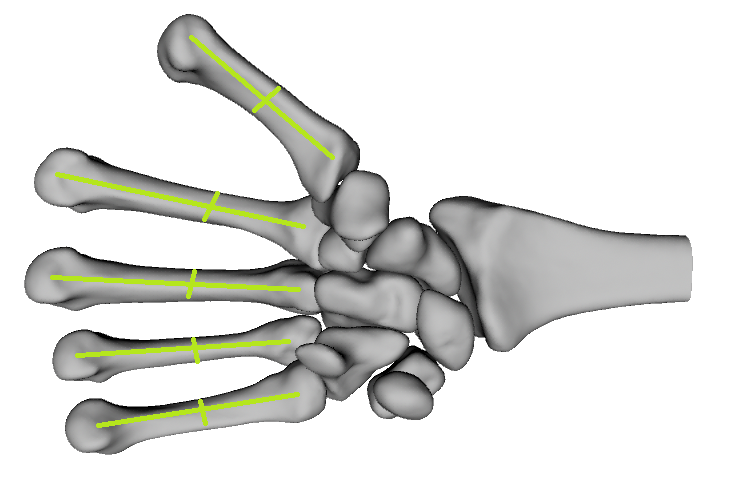
\includegraphics[valign=m,width=0.45\textwidth]{\RootDir{img/pca_shape_1-3_d.png}}
			& 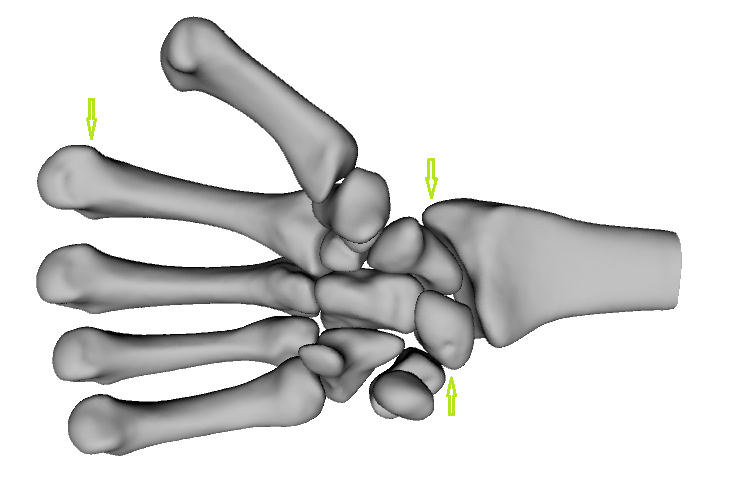
\includegraphics[valign=m,width=0.45\textwidth]{\RootDir{img/pca_shape_2-3_d.png}}
			\\ 
			
			\specialcell[c]{\textbf{Mean}\\\textbf{Shape}}
			& 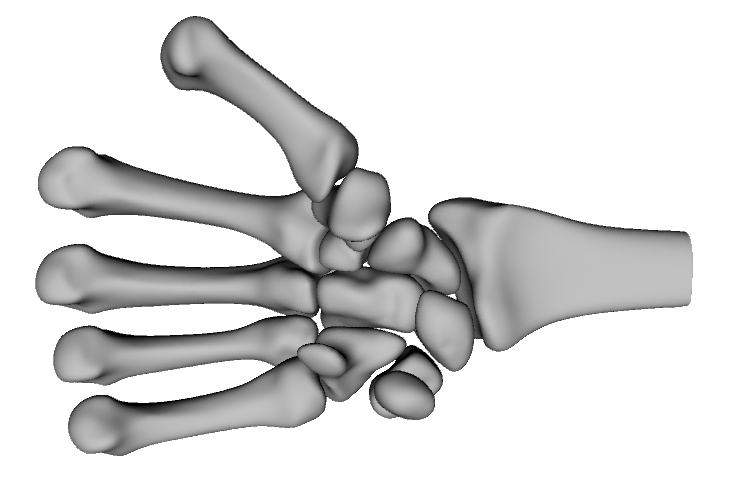
\includegraphics[valign=m,width=0.45\textwidth]{\RootDir{img/pca_mean.png}}
			& 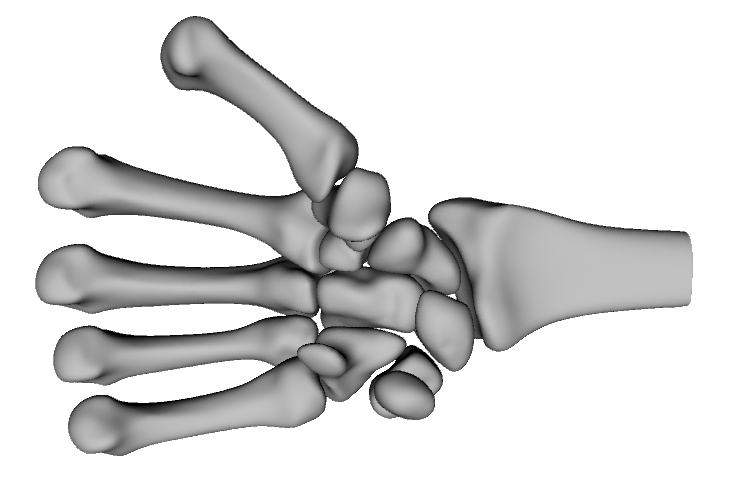
\includegraphics[valign=m,width=0.45\textwidth]{\RootDir{img/pca_mean.png}} 
			\\ 
			
			\textbf{$\mathbf{+3 SD}$}
			& 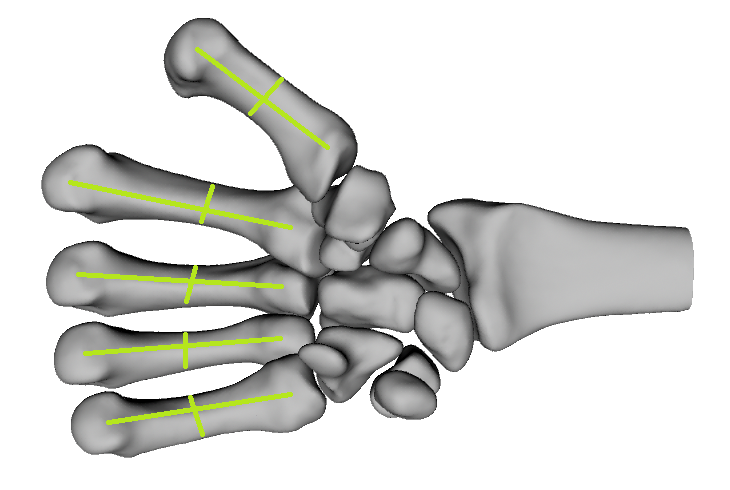
\includegraphics[valign=m,width=0.45\textwidth]{\RootDir{img/pca_shape_1+3_d.png}}
			& 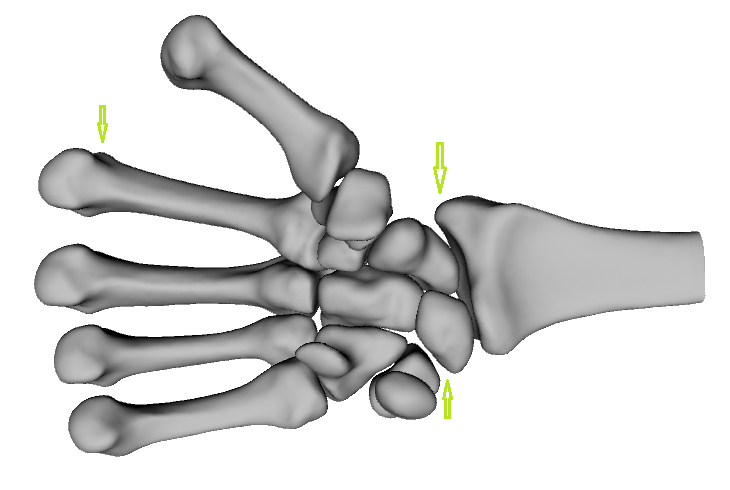
\includegraphics[valign=m,width=0.45\textwidth]{\RootDir{img/pca_shape_2+3_d.png}}
			\\
			
		\end{tabular}
		\caption[PCA results on the whole wrist]{The two principal modes of variation of the SSM including the 14 wrist bones. In the middle is shown the mean shape of the wrist bones, while above and under are illustrated the effects of the two principal modes of variation, at extreme values. In the left column is shown the most important mode, in the right the second most important one. The two modes are associated with respective variances of $17\%$ and $11\%$ of the total model variance. }
		\label{im:4_pca_whole_wrist}
	\end{adjustwidth}
	
\end{figure}


When a SSM is computed, one of the parametrization decision to make is the number of eigenvectors that should be used. When the number of data is small, the eigenvectors associated with small variance are sometimes too specific and should be associated rather with noise than with valuable information. To determine the number of eigenvectors that should be used, the models were used to approximate new shapes. The evolution of the registration accuracy compared to the number of modes used was analyzed. The new shapes outside the training set needed for such an application were obtained with a leave-one-out method: every subject of the database was by turn left out of the training shapes and the model was registered to it. Both individual models and the whole wrist one number of modes were investigated this way. 

\paragraph{Registration of the models to the subjects}

The maximum number of modes available for a model is the minimum value between the number of measurements minus one and the dimensionality of one measurement. In our case the number of subjects is the limiting factor, 43 of them were complete wrists, making 41 the maximum number of non-zero eigenvectors for the models when a subject is left out of the training set. Therefore the models were by turn registered to the target individual using $5, 10, 15, 20, 25, 30, 35, 37, 38, 39, 40, 41$ modes. The evolution of the distance between the target mesh and the registered models were computed, using both mean distance \eqref{eq:mesh_dist} and Hausdorff distance \eqref{eq:mesh_hausdorff} between meshes. The results of the individual models are shown in \figref{im:4_mean_one_nbVec} for the mean distance, in \figref{im:4_hausdorff_one_nbVec} for the Hausdorff distance. 
The results of the complete model are similarly shown in \figref{im:4_mean_all_nbVec} for the mean distance and in \figref{im:4_hausdorff_all_nbVec} for the Hausdorff distance. It must be noted that if all bones are considered at once in the model, the distances are nonetheless measured for every bone separately. 


% Si on suppose que la distribution est unimodale, alors les axes sont alignés selon les principales directions de la distribution et les modes correspondent aux principaux modes de variation des données. Si au contraire on n'a pas une distribution unimodale (des groupes se dessinent) alors on aura toujours une réduction de la dimensionalité et des directions orthogonales, mais les modes ne correspondront pas forcément aux modes de variations principaux. \cite{davies_2008_statistical}
	
Considering the individual models, one per bone, it can be noted that the registration gets strictly better when the number of modes used gets higher. No maximal value has been reached where additional modes are unhelpful due to noisy information. This is true for all bones and both mean and maximal distances. The curves presented in \figref{im:4_mean_one_nbVec} and \figref{im:4_hausdorff_one_nbVec} are strictly decreasing. We can note that the mean distance between the target mesh and the registered model is strictly smaller than $0.3$ mm for all bones when enough eigenvectors are considered in the model. The mean error made between a vertex and its closest point on the paired surface is smaller than the accuracy of the initial data (\precision* mm). The Hausdorff distance between the target and the model lies between 0.7 mm and 1.6 mm. The smallest difference is for the pisiform, which is the smallest carpal bones, with both the less complex shape of all and the smallest number of points to represent it (see \tabref{tab:3_nb_vertices}), enabling more details to be captured by the model. The highest difference is between the radius model and its target. This is due to the fact that it is the biggest bone, with the most vertices. Moreover the opened end of the radial styloid is an additional difficulty, that in spite of being taken into account in the distance measurement, has nonetheless a bad impact on the results. 


\begin{figure}[ht]
	\centering
	\includegraphics[width=0.9\textwidth]{\RootDir{img/pca_mean_one_nbVec.png}}
	\caption[Influence of the number of modes used for SSM registration - individual models - mean distance]{Influence of the number of principal modes used for the SSM registration. Each bone is captured by its individual model, every individual is by turn left out of the training set before being targeted by the models. The distance is computed between the registered model and the target meshes using a mean distance \eqref{eq:mesh_dist}. }
	\label{im:4_mean_one_nbVec}
\end{figure}


\begin{figure}[ht]
	\centering
	\includegraphics[width=0.9\textwidth]{\RootDir{img/pca_hausdorff_one_nbVec.png}}
	\caption[Influence of the number of modes used for SSM registration - individual models - Hausdorff distance]{Influence of the number of principal modes used for the SSM registration. Each bone is captured by its individual model, every individual is by turn left out of the training set before being targeted by the models. The distance is computed between the registered model and the target meshes using the Hausdorff distance \eqref{eq:mesh_hausdorff}.}
	\label{im:4_hausdorff_one_nbVec}
\end{figure}


When considering the model of the whole wrist, the results are more complex. While the distances for most of the bones between the model and the target meshes decrease with the number of modes used, for some bones they increase instead. Finally for some of them, the distance starts by increasing with the number of modes, before decreasing. It can also be observed that the curves between the mean and the Hausdorff distance in \figref{im:4_mean_all_nbVec} and \figref{im:4_hausdorff_all_nbVec} are not similar while they look a lot alike when individual models are considered. 

The bones with the most vertices, such as the radius and the metacarpals become strictly closer to the target shapes in mean distance when the number of modes increases. This is due to a stronger influence on the mean value compared to bones with less vertices. On the opposite, it can be noted that the pisiform, the bone with the less vertices has a distance strictly increasing with the number of modes used. 
For 8 bones out of 14, the mean distance between a vertex and its closest point on the paired surface is smaller than $0.32$ mm, which is also smaller than the accuracy of the original data. However for the rest of them, the mean distance is higher than $0.33$ mm. The Hausdorff distance is included in [1.1; 2.0] mm. 

The mean distance when individual models are used is below the acquisition accuracy. However the maximal distances are still high, some details are present in one person only of the database. When the latter is taken off the training set and the models are registered to its bones, these details are not captured by the model, as testified by the high maximal distances. We can conclude that a larger training set would give better results, although these are already satisfying.
Concerning the SSM modeling all wrist bones at once, the gap between the target bones and the model is too large. The number of data available are not enough for such a complex model, details are buried in the general shapes of the bones. 
It must also be noted that various profiles of people have been scanned to compose the \db*. Young and old people, males and females. However nothing guarantees that all types of wrists are present in the database, and these results rest upon the quality and diversity of the database. 

\begin{figure}[ht]
	\centering
	\includegraphics[width=0.9\textwidth]{\RootDir{img/pca_mean_all_nbVec.png}}
	\caption[Influence of the number of modes used for SSM registration - whole wrist model - mean distance]{The influence of the number of principal modes used for the SSM registration. The whole wrist is captured by the model, every individual is by turn left out of the training set before being targeted by the model. The distance is computed between the registered model and the target meshes using a mean distance \eqref{eq:mesh_dist}, the distance to each bone being separately measured, while all bones were deformed at once by a unique model. }
	\label{im:4_mean_all_nbVec}
\end{figure}

\begin{figure}[ht]
	\centering
	\includegraphics[width=0.9\textwidth]{\RootDir{img/pca_hausdorff_all_nbVec.png}}
	\caption[Influence of the number of modes used for SSM registration - whole wrist model - Hausdorff distance]{The influence of the number of principal modes used for the SSM registration. The whole wrist is captured by the model, every individual is by turn left out of the training set before being targeted by the model. The distance is computed between the registered model and the target meshes using the Hausdorff distance \eqref{eq:mesh_hausdorff}, the distance to each bone being separately measured, while all bones were deformed at once by a unique model.}
	\label{im:4_hausdorff_all_nbVec}
\end{figure}


\paragraph{Correspondence quality factors}
In a second time, we use the individual SSMs of the bones to evaluate the correspondence quality factors between the meshes $M_{W\{b,i\}}$ previously generated. Indeed we have so far only been concerned by shapes similarity (\secref{sec:4_Validation}), not correspondence between vertices. 

The evaluation of the correspondence relations proposed by Davies et al. \cite{davies_2001_minimum} (\secref{ssec:2_StateArt_Corr}) is based on the quality of the SSMs resulting from the corresponding meshes. We present the values for the 3 factors: compactness, specificity and generalization in \tabref{tab:specificity_generalization}. The factors definitions were presented in \secref{ssec:2_StateArt_Corr}.
For all factors, the lower the value is, the better. However, specificity and generalization of a model are opposite goals, one can only be improved at the expense of the other. 


%%%%%%         TABLEAU DISTANCE MESHES SPECIFICITY
% Généré à partir du script : D:/users/emilie/chirocap/prog/cmc_database/measure_res_cmc/pca/specificity_pca.py

\begin{table}[!ht]
	\centering
	\begin{tabular}{>{\RaggedRight}p{2.2cm} %centré gauche
			>{\centering\arraybackslash}p{1.6cm}
			>{\centering\arraybackslash}p{1.6cm}
			p{0.3cm}
			>{\centering\arraybackslash}p{1.6cm}
			>{\centering\arraybackslash}p{1.6cm}
%			p{0.7cm}
			>{\centering\arraybackslash}p{2.3cm}}
		\toprule
		& \multicolumn{2}{c}{\textbf{Specificity} (mm)} &&  \multicolumn{2}{c}{\textbf{Generalization} (mm)} & \textbf{Compactness}	\\
		& Dist \eqref{eq:mesh_dist} & Dist \eqref{eq:mesh_hausdorff} && Dist \eqref{eq:mesh_dist} &  Dist \eqref{eq:mesh_hausdorff} & \\
		\midrule \ \vspace{-2.5mm} & & & & &  \\
		Radius		 	& 0.202 	& \textit{1.645} && 1.052	& \textit{4.064} & 7126 \\
		Scaphoid		& 0.176 	& \textit{1.024} && 0.720 	& \textit{3.453} & 893 \\
		Lunate		 	&  0.145 	& \textit{1.117} && 0.701 	& \textit{2.873} & 579 \\
		Triquetrum		& 0.172 	& \textit{1.022} && 0.709 	& \textit{3.114} & 482 \\
		Pisiform		& 0.108 	& \textit{0.490} && 0.565 	& \textit{2.455} & 296 \\
		Trapezoid		& 0.140 	& \textit{0.857} && 0.612 	& \textit{2.574} & 648 \\
		Trapezium		& 0.213 	& \textit{0.952} && 0.639 	& \textit{3.329} & 542 \\
		Capitate		& 0.235 	& \textit{1.371} && 0.711 	& \textit{4.274} & 1261 \\
		Hamate		 	& 0.168 	& \textit{0.901} && 0.701 	& \textit{3.647} & 967 \\
		Metac. 1		& 0.182 	& \textit{1.079} && 1.033 	& \textit{3.917} & 2529 \\
		Metac. 2		& 0.228 	& \textit{1.337} && 1.023 	& \textit{3.814} & 4674 \\
		Metac. 3		& 0.225 	& \textit{1.525} && 0.985 	& \textit{5.406} & 4827 \\
		Metac. 4		& 0.175 	& \textit{1.113} && 0.889 	& \textit{3.367} & 2258 \\
		Metac. 5		& 0.077 	& \textit{0.745} && 0.861 	& \textit{3.143} & 2156 \\
		\bottomrule
	\end{tabular}
	\caption[Generalization, Specificity and Compactness of the SSMs]{Evaluation of correspondence quality based on the SSMs modeling one bone each and 39 principal modes with the three standard criteria: Generalization, Specificity and Compactness. }
	\label{tab:specificity_generalization}
\end{table}


We have computed these factors based on 39 principal modes for each individual model, one model describing one bone. The three factors are useful to compare various correspondence methods used on a same database. However, they can not be interpreted on their own. We give their values as reference, should anyone propose another set of corresponding meshes from the same database. 

PCA-models are frequently used for the modeling of 3D shapes. They are easy to compute and to employ. Such SSMs are convenient for encoding prior information about classes of shapes. However, they are linear model, and if they are robust towards noise, they can only represent shapes that are in the linear span of their training set. We propose therefore in a second phase to work with statistical models based on Gaussian Processes, which can describe a larger span of shapes from the same training set by enforcing other properties of the shapes deformations, such as smoothness.

\clearpage

%======================================
\subsection{Gaussian Processes}
\label{subsec:4_GP}

Models based on a PCA are commonly used for shape analysis and prior information for image segmentation for instance. We propose to use models based on Gaussian Processes. It rests on two observations: PCA-based models are linear, and can only represent shapes in the span of their training set. Non-linear models could widen the range of shapes that can be represented, which is especially interesting when the quantity of data available is small. Moreover the use of PCA-based models is entirely automatic, users have no possibility of intervention, even when it is clear to a human eye that the model registration results are false. It is all the more regrettable that doctors accumulate a lot of knowledge about bone shapes or image segmentation that cannot be used by the model. Gaussian processes can be used to create parametric models that are non-linear. They can also integrate knowledge provided by a user in their prior information and adapt consequently the model. 
We will firstly detail the reasons that make Gaussian Processes more adapted for modeling. Then we will briefly introduce the mathematical background (for further details, the reader is referred to 
\cite{luthi_2017_gaussian, duvenaud_2014_automatic, williams_2001_using}). Finally, we will present the two models that we have computed: a parametric one, entirely automatic and another one intended for user interaction. 

Statistical models based on a Principal Component Analysis are linear parametric models. They are very specific, due to their limited capacity of representing shapes that are necessarily in a linear span of the training set. This specificity is an upside, it makes the model robust towards artifacts and noise. However, this specificity can also be a downside when the training set is small, it jeopardizes the generalization capacity of the model \cite{luthi_2017_shape}. Yet appropriate databases can happen to be small, in particular for medical images. Furthermore, if the training data are composed of healthy subjects only, the model will be unable to characterize pathologic instances of the class. It may be enough for automatic detection of irregularities, but the model won't be able to adapt to the new instance. 
Finally these models are by nature designed to be embedded into fully automatic algorithms. The user has no control over the results. 


Gaussian Process models characterize the possible deformations of a shape based on kernels. The kernels can describe prior information based on training data, but can also be analytically created to enforce properties such as smoothness or symmetry. Multiple kernels can be combined to blend their features. The use of such customized kernels enables the non-linearity of the model, and the span of the possible shapes represented by the model is widened compared to the PCA-based model. It allows to reduce the bias induced by a limited number of instances in the training set. A second property of such a model is that depending on the kernel used, if the latter is independent of any training set, the model can describe a continuous shape independently of the points distribution. The model is also able to integrate new posterior information, and to adapt to take it into account. It enables user interaction, a human can indicate the location of some points. It can especially be handy for pathologic cases that can not be grasped by the model based on its kernel only. Additional human information for vertices wrongly registered by the model would enable the characterization of any form. Theoretically, helped with external knowledge, any accuracy of registration could be reached. The final results can be validated by the user, which enable the use of external knowledge brought by specialists.

%Even if the Gaussian Processes are widely used in different domains, the application to statistical shape models are not very widespread yet, and to our knowledge, have never been used for bone wrist shapes. Indeed 
Most existing statistical shape models of wrists are based on a Principal Components Analysis (PCA), or derivative methods. 
We propose to use a model for two applications: one fully-automatic registration of shapes, to compare with the PCA-based model, and another one fully dependent on external information: the expected corresponding final set-up is a continual interaction between the algorithm and the user, who gives any information he judges needed. 

Our work has been mostly based on Lüthi et al articles \cite{luthi_2013_unified, luthi_2017_shape, luthi_2017_gaussian}. 




%--------------------------------------
\subsubsection{What are Gaussian Processes Morphable Models (GPMM)}
\label{ssubsec:5_GP_what}

In this subsection is introduced the theory behind the GPMMs. These models were introduced by Lüthi et al. and are explained in detail in a series of articles including \cite{luthi_2017_shape, luthi_2017_gaussian}. In a first paragraph the mathematical concepts behind the models are introduced. Then in a second paragraph the models theory is described, along with various possibilities of covariance kernels and their effects for the model. 


\paragraph{Gaussian Processes}
A \textit{stochastic Process} generalizes the concept of random variable. It is composed of a collection of random variables, which all take values from the same mathematical space. Often the random variables can be indexed by some mathematical set. A \textit{Gaussian Process} is a stochastic process composed of random variables, possibly an infinity of them, such that any finite subset of these variables follows a multivariate normal distribution. The Gaussian process distribution is the joint distribution of all its random variables, and as such is a distribution over functions with a continuous domain, for example space. This property is very interesting in the case of the GPMMs as it allows to describe shape deformations as vector fields independently of the discretization. This is not the case with SSMs which are defined for a unique vertex distribution over the surface. A Gaussian process $\mathcal{GP}(\mu,k)$ is completely defined by its second-order statistics: its mean $\mu$ and its covariance $k$. 

Let us consider the covariance function $k$ of a Gaussian Process $u_t \in \mathcal{GP}(0, k)$ for $t \in \Omega$, $\Omega$ is a subset of $\mathbb{R}^d$. A linear operator $\mathcal{T}_k$ is associated to $k$ such that: 

\begin{equation}
	\begin{split}
		\mathcal{T}_k : L^2(\Omega) &\rightarrow L^2(\Omega) \\
						f &\mapsto \mathcal{T}_kf = \int_\Omega k(s,\cdot)f(s)p(s)d(s)
	\end{split}
\end{equation}

The eigenvalues and eigenfunctions pairs ($\lambda_i, \Phi_i$) of the linear operator $\mathcal{T}_k$ are found by solving the equation: 

\begin{equation}
	\label{eq:karhunen_eigenvalues}
	\int_\Omega k(s,t)\Phi_i(s) p(s) ds = \lambda_i \Phi_i(t)
\end{equation}

$p(s)$ is a density function defined on $\Omega$.
The \textit{\kl* theorem} states that a Gaussian Process can be represented as an infinite linear combination of orthogonal functions $\{\Phi_i\}_{i=1}^\infty$, its covariance's eigenfunctions:

\begin{equation}
	\label{eq:karhunen_th}
	u \sim \sum_{i=1}^{+\infty} \alpha_i \sqrt{\lambda_i} \Phi_i, \text{ \ \ \  s.t. } \alpha_i \in \mathcal{N}(0,1)
\end{equation}


On the opposite of other expansions, the orthogonal basis functions depend on the process, determined by its covariance function. The coefficients in the \kl* theorem are independent Gaussian random variables $\{\alpha_i\}_{i=1}^\infty$. Due to the latter property, the eigenvalues $\lambda_i$ explain the variance associated to the $i^{th}$ component. Therefore, if the sorted $\lambda_i$ decrease sufficiently quickly, a low rank approximation of u can be used: 

\begin{equation}
	\label{eq:karhunen_approximation}
	\tilde{u} \sim \sum_{i=1}^{r} \alpha_i \sqrt{\lambda_i} \Phi_i
\end{equation}

This approximation enables to get a parametric low-dimensional model from the Gaussian Process. The associated error is given by: 

\begin{equation}
	\sum_{i=r+1}^{\infty} \lambda_i
\end{equation}

 
The \kl* theorem is closely related to the Principal Component Analysis, since the latter is also called \kl* transform and is an empirical use of the \kl* theorem. 

The approximation \eqref{eq:karhunen_approximation} can only be used if the eigenvalues and eigenfunctions $(\lambda_i, \Phi_i)_{i=1}^r$ can be computed. Lüthi et al. propose to estimate the pairs using the Nyström method, which approximates the integral of \eqref{eq:karhunen_eigenvalues}. 
The integral over $p(x)$ is replaced by an empirical average over randomly sampled points $\{x_1,...,x_n\}$, sampled according to $p$. It leads to a matrix eigenproblem: 

\begin{equation}
	K^{(n)}U^{(n)} = U^{(n)}\Lambda^{(n)}
\end{equation}

with $K^{(n)}$ the kernel matrix such that $K_{ij}^{(n)} = k(x_i, x_j), \ i, j =1,..,n$. The columns of $U^{(n)}$ are eigenvectors, $\Lambda^{(n)}$ is a diagonal matrix with the corresponding eigenvalues $\lambda_1 \geq \lambda_2\geq ... \lambda_n \geq 0$. The Nyström approximation of the $i^{th}$ eigenfunction is: 

\begin{equation}
	\Phi_i(y) \approx \frac{\sqrt{n}}{\lambda_i^{(n)}} k_y.u_i^{(n)}
\end{equation} 

with $k_y = (k(x_1, y), ..., k(x_n, y))$ and $u_i^{(n)}$ the $i^{th}$ column of $U^{(n)}$. The eigenvalues $\lambda_i^{(n)}$ approximate the $\lambda_i$s.



%%%%%%%%%%%%%%%%%%%%%%%%%%%%%%%%%%%%%%%%%%%%%%%
\paragraph{Gaussian Process Morphable Model}

Gaussian Process Morphable Models are a generalization of more classical SSMs such as the PCA-based ones. The deformations undergone by a shape are modeled as a Gaussian Process, which is fully characterized by its mean and covariance functions. Due to the \kl* expansion of Gaussian processes and its resulting low-rank approximation, a parametric low-dimensional model describing the deformations can be computed, using the Nyström method. 

It must be noted that PCA-based models are usually employed for modeling shapes variations using a normal distribution $\mathbf{x} \sim \mathcal{N}(\bar{\mathbf{x}}, C)$, $\mathbf{x}$ being a shape. However, instead of describing shapes, SSMs can model deformations undergone by the mean shape. Let $\Delta$ be the deformations modeled, then similarly to \eqref{eq:pca_new_shape}, $\Delta =  wV^t\sqrt{\Lambda}$ and $\Delta \sim \mathcal{N}(0,C)$.
The latter interpretation is the one used for GPMMs, the probabilistic model is defined directly on the deformations undergone by the mean shape. The generation of shapes from deformations simply consists in adding the mean shape to the deformations. 

A Gaussian Process is characterized by its mean and covariance functions. The functions defining the model must be carefully chosen, as they impart its specific properties. Some such properties can enforce smoothness, periodicity, symmetry, and so on. We will only discuss two kernels that are of interest for shape deformation modeling, but many more possibilities exist, either for modeling or other applications. 

The first property that we are interested in is \textit{smoothness} of the deformations. A very simple assumption consists in using a zero mean function. It implies that the reference shape that is being deformed is a representative instance of its class of shapes, close to a mean shape. Many different kernels can be used to enforce smoothness, one of the most classical one being a Gaussian kernel: 

\begin{equation}
	\label{eq:gaussian_kernel}
	k_g(x, y) = s \cdot I_{3\times3} \cdot \exp(-||x-y||^2/\sigma^2)
\end{equation} 

% ($\Omega = \Gamma_R$ la shape de référence)
$x, y \in \Omega \subset \mathbb{R}^3$, with $\Omega = S_R$, $S_R$ being the reference surface that is being deformed. $s \in \mathbb{R}$ characterizes the scale of the deformation and $\sigma$ defines the range of influence of a point. Finally, the identity matrix $I_{3\times3}$ signifies that the 3 dimensions of the vector field are independent. 

This model incorporates no prior knowledge about a shape, and can therefore be applied to any shape, no matter its point distribution or the absence of training shapes. 
However, when a set of valid shapes are available for training, it is ideal to learn valid deformations from them. We are therefore interested in a second time in \textit{learning prior information from a training set}. If $n$ valid shapes are in correspondence, deformation fields $\Delta_1, .., \Delta_n$ can be learned from the points locations, by subtracting the mean shape points positions. A Gaussian Process $\mathcal{GP}(\mu_{p}, k_{p})$ modeling these deformations can be computed: 

\begin{equation}
	\mu_{p}(x) = \frac{1}{n} \sum_{i=1}^{n} \Delta_i(n)
\end{equation}

\begin{equation}
	k_p(x,y) = \frac{1}{n-1} \sum_{i=1}^{n} (\Delta_i(x)-\mu_p(x))(\Delta_i(y) - \mu_p(y))^T
\end{equation}

On the opposite of the Gaussian kernel, the deformation field is only known for the point distribution of the corresponding shapes. 


The only requirement for a matrix to be a valid Gaussian Process covariance function is that it should be symmetric and positive semi-definite. Algebraic rules define authorized operations between valid kernels to combine them into more complex ones. It enables the accumulation of various effects into complicated models. For example, a kernel resulting from a sum of Gaussian kernels with various $s$ and $\sigma$ values would allow multi-scale deformations, piling up global tendencies with finer and more local details. Other combinations can be used to make models more local or else to define partitions of the shape and apply various transformations depending on the section of the partition. More details about such combinations of transformations can be read in \cite{luthi_2017_gaussian}. 

We are interested in making the most of the valid shapes available in the \db*. However when the training set is limited, the span of shapes that can be represented by the model might not encompass the full shape space. In this case, the model is biased towards the training shapes. It is possible to reduce the bias by using a Gaussian kernel with parameter $\sigma$ chosen large and $s$ equal to the average error made by the prior model alone, as studied in \cite{luthi_2013_unified}. It is based on the assumption that deformations are smooth and errors are spatially correlated. Therefore, we combine the prior learned from the training set in $\mathcal{GP}(\mu_{p}, k_{p})$ with a Gaussian kernel $\mathcal{GP}(0, k_{g})$. The new model is based on a Gaussian Process $\mathcal{GP}(\mu_{p}, k_{p} + k_g)$

Another interesting property of a Gaussian Process based model is the ability to combine prior information and locations of some points given by a user to compute a new \textit{posterior model}. 
Let $\Delta$ be the deformation modeled by a Gaussian Process, describing the prior information: 

\begin{equation}
	\Delta \sim\mathcal N (\Mu, K)
\end{equation} 

If $\Delta$ is in the form of a vector, describing the deformation for a point distribution then $\Mu$ and $K$ are respectively a vector and a matrix. The most probable prior shape deformation is the mean vector $\Mu$.

The user provides the actual deformations $\delta_{\text{obs}} =  \{\delta_1,..\delta_q\}$ of points $\{p_1,..,p_q\}$. $\Delta$ can be decomposed into two vectors $\Delta_Y$ and $\Delta_Z$ such that $\Delta_Z$ describes deformations for points $\{p_1,..,p_q\}$, while $\Delta_Y$ characterizes deformations for all the other points. $\Mu$ and $K$ are decomposed accordingly: 

\begin{equation}
	\Delta = 
	\begin{pmatrix} \Delta_Y \\ \Delta_Z \end{pmatrix}
	\sim\mathcal N \Bigg(
	\begin{pmatrix} \Mu_Y \\ \Mu_Z \end{pmatrix}, 
	\begin{pmatrix} 
	K_{Y,Y} & K_{Y,Z} \\ 
	K_{Z,Y} & K_{Z,Z} 
	\end{pmatrix} 
	\Bigg)
\end{equation}

Except if $K$ is  an identity matrix, points are related to each other and the movement of one point influences its neighbors. $\Delta_Y$ is modeled by a new Gaussian Process taking the added posterior information $\delta_{\text{obs}}$ into account:

\begin{equation}
	\Delta_Y | \delta_{obs} \sim \mathcal N( \Mu', K')
\end{equation}

such that: 
\begin{equation}
	\label{eq:posterior_info_exacte}
	\begin{split}
		\Mu'(p) &= \Mu(p) + K_{p,Z} \ K_{Z,Z}^{-1} \ (\delta_{obs} - \Delta_Z) \\
		K'(p,p') &= K(p,p') - K_{p,Z} \ K_{Z,Z}^{-1} \ K_{Z,p'}
	\end{split}
\end{equation}

The posterior model of the whole shape deformations is defined in eq. \ref{eq:posterior_model}, and the most probable shapes are those characterized by the new mean. 
\begin{equation}
	\label{eq:posterior_model} 
	\begin{pmatrix} \Delta_Y \\ \Delta_Z \end{pmatrix}
	\sim\mathcal N \Bigg(
	\begin{pmatrix} \Mu_Y' \\ \delta_{obs} \end{pmatrix}, 
	\begin{pmatrix} 
		K_{Y,Y}' & 0 \\ 
		0  & 0
	\end{pmatrix} 
	\Bigg)
\end{equation} 

So far we have assumed that information given by the user are exact. It is however reasonable to suppose that it might be \textit{noisy}. Indeed 3D shape visualization on a computer is tricky and so is the definition of exactly corresponding points.
Then the observed deformations $\tilde{\delta}_\text{obs} = \{\tilde{\delta}_1,..,\tilde{\delta}_q\}$ are such that 

\begin{equation}
	\hspace*{4cm}
	\tilde{\delta}_i = \delta_i + N, 
	\hspace*{2cm} \text{s.t. } N \sim \mathcal{N}(0, \epsilon^2 I_{3\times3})
\end{equation}

$\delta_i$ is the exact deformation for point $p_i$, $\tilde{\delta}_i$ is the observed one. $N$ represents the noise and $\epsilon$ is a parameter to scale it. The prior model becomes: 

\begin{equation}
	\Delta_n = 
	\begin{pmatrix} \Delta_Y \\ \Delta_Z \end{pmatrix}
	\sim\mathcal N \Bigg(
	\begin{pmatrix} \Mu_Y \\ \Mu_Z \end{pmatrix}, 
	\begin{pmatrix} 
	K_{Y,Y} & K_{Y,Z} \\ 
	K_{Z,Y} & K_{Z,Z} + \epsilon^2 I_{3q\times3q} 
	\end{pmatrix} 
	\Bigg)
\end{equation}

and:
\begin{equation}
	\Delta_n | \tilde{\delta}_{obs} \sim \mathcal N( \Mu'_n, K'_n)
\end{equation}

such that for any points $p$, $p'$ of the shape, whether among the observed ones or not: 

\begin{equation} 
	\label{eq:noisy_posterior}
	\begin{split}
		\Mu'_n(p) &= \Mu(p) + K_{p,Z} \ (K_{Z,Z} + \epsilon^2 I_{3q\times3q})^{-1} \ (\delta_{obs} - \Delta_Z) \\
		K'_n(p, p') &= K(p, p') - K_{p,Z} \ (K_{Z,Z} + \epsilon^2 I_{3q\times3q})^{-1} \ K_{Z,p'}
	\end{split}
\end{equation}

The GPMM describes the deformations of a shape. The training set is constructed from the matrix of shapes $\mathbf{X}$ defined in \secref{ssubsec:4_PCA_what}. The matrix is centered using 
$\mathbf{X_c}(i,j) = \mathbf{X}(i,j) - \bar{\mathbf{x}}(j)$
with $\bar{\mathbf{x}}$ calculated using \eqref{eq:mean_vector}. When a new deformation is simulated with the model, the equivalent shape is generated by summing the deformation and $\bar{\mathbf{x}}$. In the following section, such a model was computed with our data, we present the results. 

%--------------------------------------
\subsubsection{Applications}
\label{ssubsec:5_GP_nowork}

We test GPMMs for 3D shape registration towards the \db* meshes \mr*. The bones are considered separately, a model only describes one bone. The registrations are done in a leave-one-out manner: the target bone is systematically removed from the training set of the model. We use two distinct strategies to register the model to the target. First, we focus on the property of the Gaussian Processes to adapt to posterior information. It is aimed at using external knowledge brought by a human user. In a second part, we will focus on an fully automatic registration method, similar to a SSM registration, based on deformation described by vectors. 


\paragraph{Registration based on external inputs}

One of the arguments in favor of a Gaussian Process-based model is the exploitation of human knowledge, to fill in potential gaps of training data. Thus, we test a registration of models to new wrists completely based on external inputs.
We have chosen to work with models based on a Gaussian Process $\mathcal{GP}(\mu_{p}, k_{p} + k_g)$ combining knowledge from training data with the assumption that deformations are smooth. \cite{luthi_2013_unified} found out that it is an efficient covariance kernel for model registration. 

The algorithm leading to model registration based on user input is:


\begin{enumerate}
	
	\item $t=0$: For a given target mesh \mr*, the corresponding model $G_{\{b,i\}}(\mu_t, k_t)$ is computed by using all \mw*, $j \in \{1, ..,n\}, j \neq i$  as training set.
	
	\item $M_{G{\{b,i\}}(\mu_t, k_t)}$ is aligned to \mr* using affine transformations. 
	
	\item The point $v_k \in G_{\{b,i\}}(\mu_t, k_t)$  with the biggest variance is computed based on $k_t$
	
	\item \textbf{User input}: The desired location for one point of $M_{G{\{b,i\}}(\mu_t, k_t)}$, whether $v_k$ or another one. The deformation is calculated from the position
	
	\item $t=t+1$: $\mu_{t}$ and $k_{t}$ are updated according to \eqref{eq:noisy_posterior}
	
	\item $d_\text{mean} (M_{G{\{b,i\}}(\mu_t, k_t)}, M_{R,\{b,i\}})$ is computed using \eqref{eq:mesh_dist}
	
	\item \textbf{User input}: "Ok" $\rightarrow$ End of the algorithm; "Nok" $\rightarrow$ Repeat 3. to 7.
\end{enumerate}

$M_{G{\{b,i\}}(\mu_t, k_t)}$ is the mesh describing the most probable shape according to the model of shape deformation. It is simply the sum of the mean mesh and the mean deformation $\mu_t$ at time $t$. 


The registration continues until the similarity of the shapes given by $d_\text{mean} (M_{G{\{b,i\}}(\mu_t, k_t)},\allowbreak M_{R,\{b,i\}})$ is considered satisfying by the external user. The user can run the algorithm until he has manually given the positions of all points forming the model. In this extreme case any shape can be described, if technically possible for the number of vertices. Hence even shapes very different from the ones in the training set can be described, such as pathologic cases that can be caused by sickness. 

To begin with, this registration method is tested with a simulated ideal user. The coordinates given by the user are supposed exact. In step $5.$ $\mu_t$ and $k_t$ are updated using \eqref{eq:posterior_info_exacte}. To give exact positions, it is assumed that the optimal registration of the model $G_{\{b,i\}}$ towards the target mesh \mr* is equal to \mw*. Additionally the user systematically provides information about the vertex that has at the moment the greatest variance according to the model's kernel. Indeed it is the point for which there is the greatest uncertainty about its deformation, and potentially the most info to learn from: it is likely to influence a bigger area around it than another point with less variance.

The number of points needed from the user to reach some similarity levels are tested with the simulated ideal user. Three distances between the target mesh and the one stemming from the model are tested: $0.3$, $0.25$ and $0.2$mm. $0.3$ mm is just below the original accuracy of the CT scans (\precision*mm). Most individual PCA-based models reach an accuracy in range $[0.2; 0.25]$ mm when they are registered to a new mesh. The registration was tested for all persons and all bones of the \db* at turn in a leave-one-out manner. The minimum number of points required correspond with the number of iterations needed to drop below the similarity levels. The average minimum number of points are presented in table \tabref{tab:nb_pts_GP}.


\begin{table}[ht]
	\centering
	\begin{tabular}{lccc}
		\toprule
		\thead{Distance max.  \\ btw. the meshes} &  $< 0.3 \text{mm}$ & $<0.25 \text{mm}$ & $<0.2 \text{mm}$   \\ 
		\midrule  \ \vspace{-1.2mm} & & & \\ 
		Radius     	& 37 & 53 & 80\\
		Scaphoid 	& 13 & 16 & 23 \\ 
		Lunate		& 11 & 15 & 23 \\
		Triquetrum	& 12 & 18 & 30 \\
		Pisiform	& 7  & 10 & 17\\
		Trapezoid	& 11 & 16 & 28 \\
		Trapezium	& 17 & 26 & 43 \\
		Capitate	& 23 & 34 & 58 \\
		Hamate		& 20 & 29 & 48 \\
		Metac. 1	& 22 & 32 & 52 \\
		Metac. 2	& 29 & 45 & 78 \\
		Metac. 3	& 27 & 37 & 65 \\
		Metac. 4	& 23 & 33 & 56 \\
		Metac. 5	& 22 & 33 & 55 \\
		
		\bottomrule
	\end{tabular}
	\caption[GPMM registration with posterior information]{Average minimum number of vertices required to reach level of similarity between a target mesh \mr* and a GPMM registered $M_{G{\{b,i\}}}$ using only posterior information} 
	\label{tab:nb_pts_GP}
\end{table}


While these numbers are not that high compared to the total number of vertices composing each bone (\tabref{tab:3_nb_vertices}), for some bones they are high when the time needed by an actual human being is considered, especially when a good similarity of shapes is expected. Manipulating 3D meshes on a 2D computer screen to accurately locate the target position of a point, even when helped by tools such as magnets is highly time consuming. The total time needed would be considerable for several tens of points. All the more so that \tabref{tab:nb_pts_GP} was computed in ideal conditions, a real user would probably need more points to reach the same similarity levels. With an actual human user, the algorithm would consider the information given as noisy. Moreover the user could decide to give locations of vertices that are more remarkable due to their location instead of filling in the ones with the most variance. 

From this experiment, we conclude that a registration method completely based on human inputs is unrealistic. It requires too much time to be convenient in real conditions. 

\paragraph{Automatic registration based on the \kl* approximation}

In a second time, GPMMs are being registered to a target mesh with an automatic optimization approach. The procedure is very similar to the PCA registration. It is aimed at comparing the results of the linear SSMs registration with ones, to compare the use of a linear model with 


The registration is based on the low rank \kl* approximation presented in \eqref{eq:karhunen_approximation}. Any deformation can be approximated by a sum of vectors balanced by their associated eigenvalues and a vector $\alpha$ weighting the importance of each vector for the current deformation. These vectors are computed from the covariance function of the Gaussian Process using the Nyström method. The automatic registration of the model to the target mesh is similar to the SSM registration: the values of $\alpha$ are optimized to minimize the difference between the target shape and the deformed template. We use the same procedure as the one presented in \cite{luthi_2017_gaussian}. The parametric form of the registration problem is the following: 

\begin{equation}
	\alpha^{*} = \argmin_{\alpha} \ \ d_\text{mean} \left(\mathbf{x}_\text{target}, \bar{\mathbf{x}} +\mu + \sum_{i=1}^{r} \alpha_i \sqrt{\lambda_i} \Phi_i \right) + \eta \sum_{i=1}^r \alpha_i^2
\end{equation}


We did not have a chance to conduct an extensive review on GPMMs registration due to a lack of time. We have heavily based our experiment on the work of Lüthy et al. We have chosen to work with parametric models of 40 vectors, to have a comparable number of vectors than the SSMs, so comparisons make more sense. One model per bone was used. Our Gaussian Processes were a composition of the estimation of an empirical model based on a training set and a Gaussian kernel to model the deformations smoothness. This composition was found to be the most effective one for registration in \cite{luthi_2013_unified}. Only one set of parameters for the Gaussian kernel was tested: in \eqref{eq:gaussian_kernel}, $\sigma$ represents the smoothness and was chosen large to model global deformations: $\sigma = 10$. $s$ defines the scale of the average error, and was chosen to be $s=0.5$. A leave-one-out approach was used, for two subjects randomly selected. The average similarity between the optimized GPMMs and the target meshes are presented in \tabref{tab:GP_registration_auto}. They are compared to the registration results of the SSMs for the two same individuals. 


\begin{table}[ht]
	\centering
	\begin{tabular}{lcc cc}
		\toprule
		& \multicolumn{2}{c}{\textbf{GPMM}} & \multicolumn{2}{c}{\textbf{SSM}} \\
		& $d_{\text{mean}}$ (mm) & $d_\text{Hausdorff}$ (mm)  & $d_{\text{mean}}$ (mm) & $d_\text{Hausdorff}$ (mm) \\ 
		\midrule  \ \vspace{-1.2mm} & & & &\\ 
		Radius		 & 0.268 & 2.950 	& 0.236 	& 1.460 \\
		Scaphoid 	 & 0.219 & 1.280 	& 0.137 	& 0.805 \\
		Lunate		 & 0.144 & 0.738 	& 0.132 	& 0.871 \\
		Triquetrum	 & 0.189 & 0.895 	& 0.151 	& 0.843 \\
		Pisiform	 & 0.181 & 0.883 	& 0.130 	& 0.732 \\
		Trapezoid	 & 0.223 & 0.987 	& 0.161 	& 0.765 \\
		Trapezium	 & 0.242 & 1.078 	& 0.156 	& 1.104 \\
		Capitate	 & 0.224 & 1.449 	& 0.204 	& 1.231 \\
		Hamate	 	 & 0.220 & 1.429 	& 0.201 	& 1.123 \\
		Metac. 1	 & 0.198 & 1.204 	& 0.178 	& 1.022 \\
		Metac. 2	 & 0.225 & 1.798 & 0.184 	& 1.668 \\
		Metac. 3	 & 0.183 & 1.142 & 0.168 	& 0.964 \\
		Metac. 4	 & 0.190 & 1.063 & 0.151 	& 0.840 \\
		Metac. 5	 & 0.182 & 0.925 & 0.055 	& 0.413 \\
		\bottomrule
	\end{tabular}
	\caption[Parametric registration of GPMM]{Distance between the target mesh and the registered GPMM based on a distance minimization of the parametric model using 40 modes. Comparison with the registration of the SSMs based on 39 modes.} 
	\label{tab:GP_registration_auto}
\end{table}


The results in \tabref{tab:GP_registration_auto} show that both models are under the $0.3$ mm threshold, though the SSM ones perform better. However, the GPMMs have not been optimized at all, only one set of parameters were tested, and there's every chances that they are not the most appropriate ones. Additionally on the opposite of the SSMs, the number of modes used by the GPMMs could also be increased, it isn't limited by the size of the training set on the opposite of the linear model. Therefore, it can be expected that with optimal models the results could be improved. 

\subsection{Discussion}

In this section we have used the dense correspondence between bones of the \db* previously computed to model the shapes variability. We have proposed two different models: one built with a PCA, another one based on Gaussian Processes. 

The PCA-based models have proven to achieve good results for the registration of new shapes outside their training set, when a different model is used for each bone. The model describing the whole wrist at once couldn't replicate the shapes with a good enough level of details. The number of modes available, depending on the number of shapes in the training set was too poor to catch all the features. 

In a second phase, Gaussian Processes were used to model the variability of the deformations undergone by the mean bone shapes. They were then registered in turn to the database meshes, using two methods: one stepwisely incorporating posterior information from a user and one based on a parametric approximation of the Gaussian processes. The first approach has proven to require too many given points to be used on real conditions with a human user though a good similarity could be reached when enough information is provided. The second approach has not been extensively tested, but achieve similar results as the SSMs while the parameters have not been optimized. It is promising, and should be further studied. 

The individual SSMs were quite effective to approximate new shapes. In the next section, they will be further tested by using them to register bones of a new database, in order to define correspondence between this second database and the CMC one. 
